\chapter{Logique de Hoare}
\label{hoare}
La logique de Hoare offre un complément aux logiques temporelles dans l'étude des réseaux de régulation génétique. Les logiques temporelles permettent de formuler et prouver des propriétés sur certains états du système en considérant les différentes évolutions possibles. L'approche utilisant la logique de Hoare est différente car elle permet de décrire l'évolution d'un système et d'obtenir par exemple des propriétés nécessaires à cette évolution. Il s'agit d'une approche nouvelle qui paraît plus adaptée à l'inférence de paramètres biologiques.
\section{Introduction}
Le dessein originel de la logique de Hoare est de définir un outil formel permettant de démontrer la validité d'un \emph{programme informatique} (ou, plus généralement, d'un algorithme informatique) utilisant le paradigme de la programmation impérative. Floyd propose un outil similaire en 1967 à l'aide d'organigrammes, et cite aussi les noms de Gorn et Perlis. Nous nous intéresserons néanmoins ici uniquement à la logique de Hoare telle que présentée par son auteur dans son article originel \cite{hoare-69}.

Cette logique repose sur la formulation de \emph{triplets de Hoare}, notés : \hbegini P \ha Q \hb R \hendi, où :
\begin{itemize}
  \item $Q$ est une instruction informatique (au sens large : il peut s'agir d'une suite d'instructions et donc d'un programme entier),
  \item $P$ et $Q$ sont deux assertions formulées en logique du premier ordre ou en logique modale.
\end{itemize}
Notons aussi que la logique de Hoare permet l'utilisation de variables (au sens informatique), qui associent un symbole (le nom de la variable) à un objet (sa valeur). Les variables peuvent être utilisées dans le programme $Q$, mais aussi nommées dans les assertions $P$ et $R$ (auquel cas elles se réfèrent bien sûr au même objet). L'écriture d'un triplet de Hoare signifie : \og Si l'assertion $P$ est satisfaite avant l'exécution du programme $Q$, et sous la condition que $Q$ se termine, alors l'assertion $R$ sera satisfaite après exécution \fg. L'assertion $P$ est donc appelée \emph{pré-condition} tandis que l'assertion $R$ est appelée \emph{post-condition}.

Il est à noter que la logique de Hoare, dans la forme que nous étudierons ici, ne suppose pas la terminaison d'un programme. Aussi, la post-condition peut ne jamais être satisfaite si le programme ne se termine pas. De même, la logique présentée à l'origine ne prenait pas en compte certains mécanismes propres à l'informatique tels que la programmation concurrente, les procédures ou les pointeurs. Plusieurs extensions de la logique de Hoare ont par la suite permis de combler ces manques, mais ne seront pas traités dans ce rapport.

\section{Construction de la logique}
\label{hoare-construction}
Afin d'offrir une logique complète, il est nécessaire de définir plusieurs axiomes et règles permettant l'interaction entre les assertions.
\subsection{Axiomes}
\label{hoare-axiomes}
L'axiome le plus simple est l'\emph{axiome du programme vide}, qui utilise en lieu de programme l'instruction vide \texttt{skip} n'effectuant aucune opération.
\begin{axiome}[Axiome du programme vide]
% Ancienne forme
%\begin{hoare}
%  $\{P\} \texttt{skip} \{P\}$
%\end{hoare}
  \hbegin P \ha \hskp \hb P \hend
\end{axiome}

La signification de cet axiome est intuitive et peut s'énoncer comme suit : \og Si l'assertion $P$ est vérifiée et que le programme est vide (\textit{i.e.} qu'il n'effectue aucune opération) alors $P$ sera aussi vraie après son exécution \fg.

Le second axiome, bien plus utilisé en pratique, est l'\emph{axiome d'affectation}, qui peut être appelé dès que l'on souhaite assigner (ou réassigner) une valeur à une variable.
\begin{axiome}[Axiome d'affectation]
%  \hbegin P \ha \hskp \hb P \hend
  \hbegin R[expr/var] \ha var \hassign expr \hb R \hend
où la syntaxe $R[expr/var]$ signifie : \og $R$ en remplaçant toute occurrence de $var$ par $expr$ \fg.
\end{axiome}

Cet axiome possède donc la signification suivante : \og Si l'assertion $R$ dont on a remplacé toute occurrence de $var$ par $expr$ est vraie avant l'exécution de l'affectation de l'expression $expr$ à la variable $var$, alors $R$ sera vraie après son exécution \fg. Afin d'illustrer cet axiome et de donner un premier exemple concret d'application de la logique de Hoare, considérerons le cas de l'incrémentation d'une variable :
  \hbegin y + 1 \geq 5 \ha y \hassign y + 1 \hb y \geq 5 \hend
Dans cet exemple, $y$ tient lieu de variable et $y + 1$ tient lieu d'expression. On peut naturellement simplifier la pré-condition et parvenir à la forme :
  \hbegin y \geq 4 \ha y \hassign y + 1 \hb y \geq 5 \hend
  %\begin{hoare}$\{y \geq 4\} y := y + 1 \{y \geq 5\}$\end{hoare}

Notons que l'expression $expr$ de l'axiome peut faire entrer en jeu la variable $var$ à laquelle elle sera affectée (comme c'est le cas dans l'exemple précédent) mais aussi d'autres variables ou encore des constantes.

Il est aussi intéressant de constater que dans le cas de cet axiome, la pré-condition dépend fortement de la post-condition (elle n'est finalement que le résultat d'une substitution appliquée à la post-condition). Cela permet ainsi aisément de savoir quelle pré-condition imposer pour obtenir une post-condition voulue, l'instruction d'affectation étant connue.

\subsection{Règles}
Les règles permettent de lier les triplets de Hoare entre eux et de définir des structures algorithmiques plus complexes que le simple déroulement d'un programme linéaire. Contrairement aux axiomes, certaines propriétés sont requises afin qu'elles puissent s'appliquer.

Les \emph{règles de conséquence} permettent de restreindre une pré-condition ou d'élargir une post-condition. Elles s'énoncent comme suit :
\begin{regle}[Règles de conséquence]
\begin{listesanspuce}
  \item Si \hbegini P \ha Q \hb R \hendi{} et $(R \Rightarrow S)$ alors \hbegini P \ha Q \hb S \hendi
  \item Si \hbegini P \ha Q \hb R \hendi{} et $(S \Rightarrow P)$ alors \hbegini S \ha Q \hb R \hendi
\end{listesanspuce}
%\begin{hoare}
%  $Si \{P\} Q \{R\} et (R \Rightarrow S) alors \{P\} Q \{S\}$
%  \item $Si \{P\} Q \{R\} et (S \Rightarrow P) alors \{S\} Q \{R\}$
%\end{hoare}
\end{regle}

La \emph{règle de séquence}, dite encore \emph{règle de composition}, permet d'enchaîner l'exécution de deux programmes dont les triplets de Hoare le permettent, afin d'obtenir un programme plus important :
\begin{regle}[Règle de composition]
\begin{listesanspuce}
  \item Si \hbegini P \ha Q_1 \hb R \hendi{} et \hbegini R \ha Q_2 \hb S \hendi{} alors \hbegini P \ha Q_1 ; Q_2 \hb S \hendi
\end{listesanspuce}
%\begin{hoare}
%  $Si \{P\} Q_1 \{R\} et \{R\} Q_2 \{S\} alors \{P\} Q_1 ; Q_2 \{S\}$
%\end{hoare}
\end{regle}

La \emph{règle de condition} permet l'introduction de la structure de contrôle conditionnelle (de type \textit{Si-Alors-Sinon}), tandis que la \emph{règle d'itération} permet l'introduction de la boucle répétitive conditionnelle (de type \textit{Tant que}). Elles s'énoncent comme suit :
\begin{regle}[Règle de condition]
\begin{listesanspuce}
  \item Si \hbegini P \wedge C \ha Q_1 \hb R \hendi{} et \hbegini P \wedge \neg C \ha Q_2 \hb R \hendi
  \item \quad alors \hbegini P \ha \hif C \hthen Q_1 \helse Q_2 \hfi \hb R \hendi
\end{listesanspuce}
%\begin{hoare}
%  $Si \{P \wedge C\} S1 \{Q\} et \{P \wedge \neg C\} S2 \{Q\} alors \{P\} Si (C) Alors\_Faire S1 Sinon\_Faire S2 Fin\_Si \{Q\}$
%\end{hoare}
\end{regle}
\begin{regle}[Règle d'itération]
\begin{listesanspuce}
  \item Si \hbegini P \wedge C \ha Q \hb P \hendi
  \item \quad alors \hbegini P \ha \hwhile C \hdo Q \hod \hb P \wedge \neg C \hendi
\end{listesanspuce}
%\begin{hoare}
%  $Si \{P \wedge C\} S \{P\} alors \{P\} Tant\_Que (C) Faire S Fin\_Tant\_Que \{P \wedge \neg C\}$
%\end{hoare}
\end{regle}

Il est intéressant de noter la présence de l'assertion $P$ dans la pré-condition et dans la post-condition de la boucle (ainsi que de son contenu seul). Cette assertion est appelée invariant, et nécessite d'être judicieusement choisie pour pouvoir effectuer les preuves.

\section{Exemple d'utilisation}
\label{hoare-exemple}
Afin d'utiliser les règles et les axiomes vus dans la section précédente, intéressons-nous à l'exemple suivant, inspiré de \cite{moeller-04}.%\\
\vspace{0.1cm}
%\begin{singlespace}
\begin{spacing}{0.7}
\hbegin t \geq 0 \hal
  \hitem $n \hassign t;$
  \hitem $r \hassign 1;$
  \hitem $\hwhile n \neq 0 \hdo$
  \hitem    \quad$r \hassign r \times n;$
  \hitem    \quad$n \hassign n - 1;$
  \hitem\!\!$\hod$;
\hbl r = t! \hend
\end{spacing}%\ \\
~\vspace{0.1cm}

%\end{singlespace}\ \\

%$$\{t \geq 0\}$$
%\begin{lstlisting}
%n := t;
%r := 1;
%Tant_Que n \neq 0 Faire
%   r := r * n;
%   n := n - 1;
%Fin_Tant_Que 
%\end{lstlisting}
%$$\{r = t!\}$$

Afin de démontrer le triplet de Hoare ci-dessus, il suffit de procéder par étapes successives, en prouvant des propriétés sur chacune des lignes grâce aux règles et à l'axiome d'affectation. Il sera alors possible de regrouper les triplets ainsi obtenus à l'aide des règles de conséquence et de composition pour démontrer la propriété globale du programme.
Commençons par la première ligne. d'après l'axiome d'affectation, son exécution vérifie :
  \hbegin t \geq 0 \wedge t = t \ha n := t; \hb t \geq 0 \wedge t = n \hend
Soit, après simplification de la pré-condition et substitution de $n$ à $t$ dans la post-condition :
  \hbegin t \geq 0 \ha n := t; \hb n \geq 0 \wedge t = n \hend
De même, toujours d'après l'axiome d'affectation, l'exécution de la ligne~2 vérifie le triplet de Hoare suivant (après simplification) :
  \hbegin n \geq 0 \wedge t = n \ha r := 1; \hb n \geq 0 \wedge t = n \wedge r = 1 \hend
La post-condition du premier triplet est ainsi identique à la pré-condition du second triplet. Nous pouvons alors directement composer les deux programmes pour obtenir un unique triplet de Hoare :
  \hbegin t \geq 0 \ha n := t; r := 1; \hb n \geq 0 \wedge t = n \wedge r = 1 \hend \doublespacing

\singlespacing La partie d'initialisation étant traitée, il reste à considérer le c\oe ur du programme, à savoir les lignes 3 à 6, qui forment une boucle répétitive\footnote{Notons que l'instruction de la ligne~6 n'en est pas véritablement une ; en réalité elle ne sert qu'à effectuer un branchement pour terminer la structure de contrôle \textit{Tant que}.}. Prenons en compte séparément les deux lignes au sein de cette boucle. La ligne~4 vérifie :
  \hbegin r = \frac{t!}{n!} \wedge t \geq n \wedge n > 0 \ha r := r * n; \hb r = \frac{t!}{(n - 1)!} \wedge t \geq n \wedge n > 0 \hend
tandis que l'instruction de la ligne~5 vérifie :
  \hbegin r = \frac{t!}{(n-1)!} \wedge t \geq n \wedge n > 0 \ha n := n - 1; \hb r = \frac{t!}{n!} \wedge t \geq n \wedge n \geq 0 \hend
Les post-conditions ont été choisies de façon \og raisonnée \fg{} de façon à entraîner des pré-conditions qui coïncideront entre elles et avec la suite. On peut alors réunir les deux lignes contenues dans la boucle pour obtenir :
  \hbegin r = \frac{t!}{n!} \wedge t \geq n \wedge n \geq 0 \wedge n \neq 0 \ha r := r * n; n := n - 1; \hb r = \frac{t!}{n!} \wedge t \geq n \wedge n \geq 0 \hend \doublespacing

\singlespacing Toutes les instructions contenues dans la boucle se trouvent dans ce triplet de Hoare. La pré-condition a été reformulée de façon à clairement faire apparaître un invariant (une partie de l'assertion que l'on retrouve dans la post-condition) qui est : \og $r = \frac{t!}{n!} \wedge t \geq n \wedge n \geq 0$ \fg. En revanche, le reste de l'assertion ($n \neq 0$) ne se trouve que dans la pré-condition, et aura donc le rôle de condition d'arrêt pour la boucle. On peut donc appliquer la règle relative à l'itération :
  \hbegin r = \frac{t!}{n!} \wedge t \geq n \wedge n \geq 0 \ha
  $\hitem$ \hwhile n \neq 0 \hdo r := r * n; n := n - 1; \hod;
  \\ \hb r = \frac{t!}{n!} \wedge t \geq n \wedge n \geq 0 \wedge n = 0 \hend
Ici, la post-condition se simplifie naturellement en : \og r = t! \fg, ce qui est bien la post-condition finale que l'on cherche à obtenir.
Pour finir, il ne nous reste plus qu'à constater (naïvement) que :
$$(n \geq 0 \wedge t = n \wedge r = 1) \Rightarrow (r = \frac{t!}{n!} \wedge t \geq n \wedge n \geq 0)$$
D'après les règles de conséquence et de composition, on peut alors réunir le triplet de l'initialisation (lignes 1 et 2) et celui caractérisant la boucle (lignes 3 à 6). On obtient finalement le triplet à démontrer.

\section{Plus faible pré-condition et de plus forte post-condition}
L'une des principales difficultés lors de l'utilisation de la logique de Hoare est de trouver les pré-conditions et post-conditions adéquates. En effet, prouver un programme à l'aide de cette logique nécessite de le décomposer en instructions élémentaires afin de se ramener aux règles ou axiomes de la logique (ou d'utiliser des portions de codes ou des fonctions dont a déjà prouvé le comportement). Or si l'une des deux conditions du triplet est mal choisie, l'utilisation de la règle de composition est rendue impossible.

Ce cas de figure peut survenir lorsqu'un triplet de Hoare décrit un comportement plus faible que nécessaire. L'une des assertions au moins (pré-condition ou post-condition) est alors trop faible pour permettre de continuer la démonstration (car ne permet pas, par exemple, d'utiliser la règle de composition). Considérons pour illustrer cela l'exemple de triplet de Hoare présenté à la sous-section~\ref{hoare-axiomes} :
  \hbegin y \geq 4 \ha y \hassign y + 1 \hb y \geq 5 \hend
Les deux triplets suivants, utilisant le même programme, sont aussi satisfaits, mais leur signification est plus faible :
  \hbegin y = 4 \ha y \hassign y + 1 \hb y \geq 5 \hend
  \hbegin y \geq 4 \ha y \hassign y + 1 \hb y \geq 0 \hend
Dans le premier cas, la pré-condition a été restreinte à l'unique cas où $y = 4$ avant l'exécution du programme ; l'ensemble des cas d'exécutions couverts par ce triplet est donc beaucoup moins important (et en réalité réduit à une seule exécution possible). De même, le second triplet traite les mêmes cas d'exécution que le triplet d'origine, mais sa post-condition est plus faible ; il serait donc insuffisant pour une preuve nécessitant que $y \geq 5$ à la fin de cette instruction.

De façon plus générale, il est nécessaire d'éviter dans les preuves de trop restreindre la pré-condition, ou trop étendre la post-condition si on veut conserver le pouvoir d'expression de cette logique. Les cas extrêmes seraient les suivants :
  \hbegin \texttt{faux} \ha Q \hb R \hend
  \hbegin P \ha Q \hb \texttt{vrai} \hend
Ces deux triplets sont corrects : la pré-condition du premier n'est jamais satisfaite (et le triplet caractérise donc un ensemble vide de cas d'exécution), tandis que la post-condition du second l'est toujours\footnote{Il faut rappeler que la forme \og faible \fg{} de la logique de Hoare développée ici ne présuppose en rien de la terminaison des programmes ; dans le cas d'une logique \og forte \fg{}, le résultat serait différent.}. Ces deux triplets n'apportent aucune information concernant leur programme et seraient inutiles au sein d'une preuve.\\

Ces deux cas extrêmes et les exemples qui les précèdent illustrent la nécessité d'un outil permettant de maximiser le pouvoir d'expression des triplets de Hoare. Ainsi, pour un programme donné et connaissant la pré-condition d'un triplet, on souhaite pouvoir retrouver la plus forte post-condition ; de même, connaissant le programme et la post-condition, on souhaite retrouver la pré-condition couvrant le plus de cas d'exécution possibles, qui est donc la plus faible pré-condition. Cela nous amène donc à la définition des deux opérateurs ci-dessous, appelés aussi transformateurs de prédicats \cite{dijkstra-75,moeller-04}.

\subsection{Définition et propriétés}
\begin{definition}[Plus faible pré-condition et plus forte post-condition]\ 
\begin{itemize}
  \item Pour un programme $Q$ et une post-condition $R$ donnés, la plus faible pré-condition, notée $\mathrm{WP}(Q, R)$, est l'assertion la plus large possible pour laquelle $Q$ se termine et $R$ est satisfaite après exécution de $Q$.
  \item Pour un programme $Q$ et une pré-condition $P$ donnés, la plus forte post-condition, notée $\mathrm{SP}(P, Q)$, est l'assertion la plus restreinte possible qui soit satisfaite après exécution de $Q$, si $P$ est vraie avant, et sous réserve de terminaison de $Q$.
\end{itemize}
\end{definition}

Il est à noter que ces opérateurs comportent la notion de terminaison du programme. Bien que la forme de la logique de Hoare présentée ici ne présume en rien de la terminaison des programmes étudiés, la notion de plus faible pré-condition est plus restrictive\footnote{Il en existe une version moins restrictive qui diffère peu, mais elle ne sera pas étudiée ici.}.

Il est possible de montrer certaines propriétés sur les opérateurs définis ci-dessus. Pour commencer, on peut donner une caractérisation très générale des opérateurs WP et SP.
\begin{propriete}[Caractérisation de WP et SP]
\begin{listesanspuce}
  \item $($\hbegini P \ha Q \hb R \hendi $\text{ et $Q$ se termine}) \Leftrightarrow (P \Rightarrow \mathrm{WP}(Q, R)) \Leftrightarrow (\mathrm{SP}(P, Q) \Rightarrow R)$
\end{listesanspuce}
\end{propriete}

Dans la suite, nous nous intéresserons uniquement à l'opérateur de plus faible pré-condition : WP. L'opérateur SP ne sera pas traité car il ne sera pas utilisé pour rattacher la logique de Hoare aux réseaux de régulation génétiques. De plus, grâce à la forme de la règle d'affectation, la plus faible pré-condition d'une instruction d'affectation est toujours exactement connue, ce qui renforce l'intérêt pour cet opérateur.\\

D'autres propriétés peuvent être démontrées sur l'opérateur de plus faible pré-condition. Cet opérateur est dit monotone, conjonctif et disjonctif, ce qui s'exprime formellement par les propriétés suivantes.
\begin{propriete}[Monotonie de WP]
Si $R$ et $S$ sont deux assertions telles que $R \Rightarrow S$, alors pour tout programme $Q$ :
\begin{listesanspuce}
  \item $\mathrm{WP}(Q, R) \Rightarrow \mathrm{WP}(Q, S)$
\end{listesanspuce}
\end{propriete}
\begin{propriete}[Conjonction de WP]
Si $R$ et $S$ sont deux assertions, alors pour tout programme $Q$ :
\begin{listesanspuce}
  \item $\mathrm{WP}(Q, R) \wedge \mathrm{WP}(Q, S) \equiv \mathrm{WP}(Q, R \wedge S)$
\end{listesanspuce}
\end{propriete}
\begin{propriete}[Disjonction de WP]
Si $R$ et $S$ sont deux assertions, alors pour tout programme $Q$ :
\begin{listesanspuce}
  \item $\mathrm{WP}(Q, R) \vee \mathrm{WP}(Q, S) \equiv \mathrm{WP}(Q, R \vee S)$
\end{listesanspuce}
\end{propriete}


\subsection{Règles}
Les règles et axiomes de la logique de Hoare (définis à la section \ref{hoare-construction}) aident à construire le résultat de ces opérateurs. Nous allons dans la suite définir le résultat de l'opérateur WP pour certaines structures.

\begin{regle}[Plus faible pré-condition de la composition]
%La plus faible pré-condition de deux instructions composées est :
\begin{listesanspuce}
  \item $\mathrm{WP}(Q_1 ; Q_2, R) \equiv \mathrm{WP}(Q_1, \mathrm{WP}(Q_2, R))$
\end{listesanspuce}
\end{regle}

Cette règle permet de traduire la composition de deux instructions en une composition de l'opérateur WP.

\begin{regle}[Plus faible pré-condition de l'affectation]
%La plus faible pré-condition d'une instruction d'affectation est :
\begin{listesanspuce}
  \item $\mathrm{WP}(var \hassign expr, R) \equiv R[expr/var]$
\end{listesanspuce}
\end{regle}

De la même façon que pour l'axiome d'affectation, l'expression $R[expr/var]$ signifie : \og $R$ en remplaçant toute occurrence de $var$ par $expr$ \fg. On retrouve donc une formulation très proche de la règle d'affectation. On peut rattacher cela au fait que l'axiome d'affectation se définit \textit{à rebours} : la pré-condition est obtenue à partir de la forme de la post-condition.

\begin{regle}[Plus faible pré-condition de la structure conditionnelle]
%La plus faible pré-condition d'une structure conditionnelle de type \textit{Si} est :
\begin{listesanspuce}
  \item $\mathrm{WP}(\hif C \hthen Q_1 \helse Q_2 \hfi, R) \equiv C \Rightarrow \mathrm{WP}(Q_1, R) \wedge \neg C \Rightarrow \mathrm{WP}(Q_2, R)$
\end{listesanspuce}
\end{regle}

Cette formule fait clairement apparaître les deux cas distincts où $C$ est satisfaite et où elle ne l'est pas, et dépend des plus faibles pré-conditions des deux chemins d'exécution possibles.

\begin{regle}[Plus faible pré-condition de la structure itérative]
%La plus faible pré-condition d'une structure répétitive de type \textit{Tant que} est :
\begin{listesanspuce}
  \item $\mathrm{WP}(\hwhile C \hdo Q \hod, R) \equiv \exists n \geq 0, H_n$
  \item \quad où : $\left\{
\begin{array}{l}
  H_0 \equiv \neg C \wedge R \\
  \forall k \in \mathbb{N}, H_{k+1} \equiv H_0 \vee \mathrm{WP}(Q, H_k)
\end{array}
\right.$
\end{listesanspuce}
\end{regle}
Cette formule prend en compte la succession des exécutions de l'intérieur de la boucle (ici, le programme $Q$) et le fait que la boucle termine un jour (ce qui est nécessaire à la terminaison du programme ; cela se traduit par le quantificateur d'existence $\exists$).

\section{Application aux réseaux de régulation génétique}
Afin de montrer l'utilité du rapprochement entre la logique de Hoare et le formalisme de Thomas (traité au chapitre~\ref{rrg}), il est intéressant d'effectuer une comparaison avec les logiques temporelles. La logique CTL*, comme illustré au chapitre précédent, permet d'étudier les chemins possibles dans un graphe et les propriétés rencontrées sur ces chemins. Ainsi, pour un graphe d'états obtenu à partir d'un réseau de régulation génétique donné, on est en mesure de savoir quelles sont les configurations accessibles par le système de gènes modélisé. La recherche inverse est aussi possible : il existe des model-checkers\footnote{On peut par exemple citer Roméo pour les réseaux de Petri temporels paramétriques, ou PHAVer pour les automates hybrides.} qui, partant d'une propriété, sont capables d'exhiber des conditions sur la paramétrisation pour que cette propriété soit vérifiée. Cependant, cette méthode nécessite soit d'être exécutée à la volée, soit de calculer complètement le graphe d'états, qui est soumis au problème de l'explosion combinatoire.

Pour obtenir des résultats par exemple sur la paramétrisation de graphes d'interaction de grande taille, il est nécessaire que la logique utilisée travaille directement sur le réseau de régulation (et non sur le graphe d'états qui en est déduit). La logique de Hoare répond à cette nécessité à condition d'adapter le formalisme utilisé par le modèle de Thomas. Ainsi, les deux instructions admises seraient l'incrémentation et la décrémentation du niveau d'expression d'un gène, tandis que les éléments constituant les conditions porteraient sur les niveaux d'expression des gènes et sur les valeurs de la paramétrisation. Nous allons brièvement décrire ce formalisme détaillé dans \cite{khalis-bernot-comet-richard-roux-siebert-UnPublished} et expliquer son utilisation.

\begin{definition}[Comparaison atomique]
Une \emph{comparaison atomique} sur un réseau de régulation est une expression du type : \og $a \bowtie b$ \fg{} où $\bowtie$ est l'un des opérateurs de comparaison parmi $=$, $>$, $\geq$, $<$, $\leq$, et $a$ et $b$ peuvent indépendamment être :
\begin{itemize}
  \item une constante dans $\mathbb{N}$,
  \item le niveau d'expression d'un gène $v$ du graphe d'interaction\footnote{On confond souvent, pour des raisons de simplicité d'écriture, le nom d'un gène dans le graphe d'interaction avec le nom de son niveau d'expression.},
  \item une valeur $k_{v, \omega}$ de la paramétrisation $\mathcal{K}$ du réseau de régulation.
\end{itemize}
\end{definition}

%\begin{definition}[Assertion de chemin]
%Une \emph{assertion de chemin} sur un réseau de régulation est une assertion composée uniquement de comparaisons atomiques et d'opérateurs logiques de négation $\neg$ et conjonction $\wedge$.
%\end{definition}

\begin{definition}[Assertion de chemin]
Une \emph{assertion de chemin} $A$ sur un réseau de régulation est une assertion définie inductivement :
\begin{itemize}
  \item si $A \equiv a$, où $a$ est une comparaison atomique, alors $A$ est satisfaite ssi $a$ est satisfaite,
  \item si $A \equiv \neg B$ où $B$ est une assertion de chemin, alors $A$ est satisfaite ssi $B$ n'est pas satisfaite,
  \item si $A \equiv B_1 \wedge B_2$ où $B_1$ et $B_2$ sont deux assertions de chemin, alors $A$ est satisfaite ssi $B_1$ et $B_2$ sont toutes deux satisfaites.
\end{itemize}
\end{definition}

Notons que l'on peut naturellement aussi utiliser les autres connecteurs logiques, car ils se définissent tous à partir de la négation et de la conjonction.\\

On peut définir trois notations concernant les assertions de chemin, qui seront utilisées dans la suite. On rappelle que pour un gène $v$% et un état $\eta$ du système de gènes
, $b_v$ est son plafond et $G^{-1}(v)$ est l'ensemble de ses prédécesseurs dans le graphe d'interaction%$\rho(v, \eta)$ représente l'ensemble des ressources de $v$, et $d(v)$ est sa fonction de direction. 
; de plus, pour tout multiplexe $m$, $\varphi_m$ est l'assertion qui lui est associée. Pour toute variable $v$ et tout sous-ensemble $\omega$ de $G^{-1}(v)$, on note :
  $$\Phi^{\omega}_v \equiv ( \bigwedge_{m \in \omega} \varphi_m ) \wedge ( \bigwedge_{m \in G^{-1}(v) \setminus \omega} \neg \varphi_m )$$
La signification de $\Phi^{\omega}_v$ est que l'ensemble des ressources de $v$ est exactement l'ensemble $\omega$. De plus, pour toute variable $v$, on note :
  $$\Phi^+_v \equiv (0 \leq v) \wedge (v < b_v) \wedge (\bigwedge_{\omega \subset G^{-1}(v)} (\Phi^{\omega}_v \Rightarrow k_{v, \omega} > v))$$
  $$\Phi^-_v \equiv (0 < v) \wedge (v \geq b_v) \wedge (\bigwedge_{\omega \subset G^{-1}(v)} (\Phi^{\omega}_v \Rightarrow k_{v, \omega} < v))$$
%\begin{listesanspuce}
%  \item $\Phi^{\omega}_v \equiv \rho(v, \eta) = \omega$
%  \item $\Phi^+_v \equiv d(v) = +1$
%  \item $\Phi^-_v \equiv d(v) = -1$
%\end{listesanspuce}
La signification intuitive de $\Phi^+_v$ (resp. $\Phi^-_v$) est qu'il est possible d'incrémenter $v$ (resp. de décrémenter $v$) dans l'état courant car la paramétrisation et les ressources de $v$ le permettent. Les états ne sont pas précisés dans ces formules car elles seront utilisées en tant que pré-conditions et post-conditions, et donc à un instant théoriquement connu dans l'évolution du système.\\

Les programmes de chemin se définissent simplement en réutilisant les règles et axiomes de la logique de Hoare définies à la section~\ref{hoare-construction}, sauf pour l'instruction d'affectation qui devient une instructions du type : \og $v \diamond$ \fg{} où $v$ est le nom d'un gène du système et $\diamond$ représente l'action d'incrémentation (notée $+$) ou de décrémentation (notée $-$) de ce gène. On définit alors deux nouvelles règles spécifiques à ce type d'instruction.

\begin{regle}[Règles d'incrémentation et de décrémentation]
\begin{listesanspuce}
  \item \hbegini \Phi^+_v \wedge R[v+1/v] \ha v+ \hb R \hendi
  \item \hbegini \Phi^-_v \wedge R[v-1/v] \ha v- \hb R \hendi
\end{listesanspuce}
\end{regle}

On doit de plus définir le résultat de l'opérateur de plus faible pré-condition pour ce type d'instructions. Ce résultat est similaire à celui obtenu pour l'opération d'affectation, mais il faut aussi ajouter la condition d'incrémentation ou de décrémentation.

\begin{regle}[Plus faibles pré-conditions d'incrémentation et décrémentation]
\begin{listesanspuce}
  \item $\mathrm{WP}(v+, R) \equiv \Phi^+_v \wedge R[v/v+1]$
  \item $\mathrm{WP}(v-, R) \equiv \Phi^-_v \wedge R[v/v-1]$
\end{listesanspuce}
\end{regle}

Les plus faibles pré-conditions des autres instructions ou structures sont identiques à celles définies pour la logique de Hoare classique.

\subsection*{Exemple}
\begin{figure}[ht]
  \centering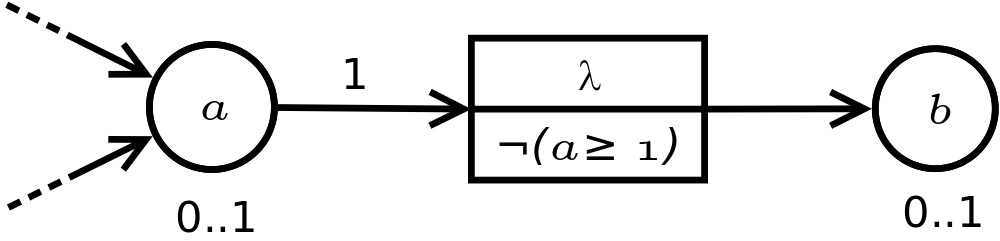
\includegraphics[width=7cm]{figs/ex-hoare-rrg}
  \caption{Un graphe d'interaction partiel. On suppose que le gène $b$ n'est influencé que via le multiplexe $\lambda$, mais que le gène $a$ peut être influencé par d'éventuels autres gènes dans le graphe.}
  \label{hoare-ex-hoare-rrg}
\end{figure}

Afin d'illustrer ce nouveau formalisme, considérons le graphe d'interaction de la figure~\ref{hoare-ex-hoare-rrg}. On suppose que d'autres gènes peuvent influer sur $a$, mais pas sur $b$.
On cherche à savoir s'il existe pour ce graphe une paramétrisation qui accepte que $b$ soit incrémenté si le niveau d'expression de $a$ est à $0$. Pour cela, on considérera le triplet de Hoare suivant :
  \hbegin a = 0 \wedge b = 0 \ha b+ \hb b = 1 \hend
On se place ainsi dans une configuration initiale où les niveaux d'expression de $a$ et $b$ sont nuls, et le chemin consiste simplement en une incrémentation de $b$. Ce triplet est intuitivement vérifié (cela sera prouvé par la suite) mais il n'est pas assez expressif. Nous allons donc utiliser l'opérateur de plus faible pré-condition afin d'obtenir des informations sur la paramétrisation nécessaire pour obtenir un tel comportement. Le résultat est la conjonction $R$ suivante :
\begin{listesanspuce}
\item $R \equiv \left\{\begin{array}{l}
  \Phi^+_b\\
  b = 0
\end{array}\right.$
\end{listesanspuce}
Lorsqu'on on décompose $\Phi^+_b$ on obtient :
\begin{listesanspuce}
\item $R \equiv \left\{\begin{array}{l}
  0 \leq b\\
  b < b_b\\
  \Phi^{\emptyset}_b \Rightarrow k_{b, \emptyset} > b\\
  \Phi^{\{\lambda\}}_b \Rightarrow k_{b, \{\lambda\}} > b\\
  b = 0
\end{array}\right.$
\end{listesanspuce}
Comme le multiplexe $\lambda$ est le seul prédécesseur de $b$, $\Phi^{\emptyset}_b$ et $\Phi^{\{\lambda\}}_b$ s'écriront uniquement en fonction de l'assertion portée par $\lambda$. Comme $\Phi^{\{\lambda\}}_b$ caractérise le cas où l'assertion de $\lambda$ est satisfaite, et $\Phi^{\emptyset}_b$ caractérise le cas contraire, on a :
\begin{listesanspuce}
  \item $\begin{array}{llrlr}
  \Phi^{\{\lambda\}}_b &\equiv& \varphi_{\lambda} &\equiv& \neg (a \geq 1)\\
  \Phi^{\emptyset}_b &\equiv& \neg \varphi_{\lambda} &\equiv& \neg\neg (a \geq 1)
\end{array}$
\end{listesanspuce}
On obtient donc en remplaçant et après simplification :
\begin{listesanspuce}
\item $R \equiv \left\{\begin{array}{l}
  b = 0\\
  (a = 1) \Rightarrow k_{b, \emptyset} > 0\\
  (a = 0) \Rightarrow k_{b, \{\lambda\}} > 0\\
\end{array}\right.$
\end{listesanspuce}
Ce résultat traduit le fait que si on souhaite incrémenter $b$ lorsque son niveau d'expression est nul, alors sa paramétrisation associée ne doit pas être égale à zéro. On retrouve donc l'une des propriétés intrinsèques au modèle de Thomas.

On peut tout d'abord constater que le triplet de départ \hbegini a = 0 \wedge b = 0 \ha b+ \hb b = 1 \hendi{} était effectivement correct, car on a bien :
\begin{listesanspuce}
  \item $a = 0 \wedge b = 0 \Rightarrow R$
\end{listesanspuce}
De plus, on peut extraire de $R$ l'information recherchée : en effet, si on suppose $a$ nul à l'état initial, on trouve la condition nécessaire suivante sur la paramétrisation : $k_{b, \{\lambda\}} > 0$.\\

Ce cas volontairement très simple illustre le fonctionnement de ce croisement entre formalismes. Il permet d'obtenir des conditions sur des cas plus complexes, mais permet aussi de déterminer le caractère réalisable ou non d'un chemin. Par exemple, le chemin $b+ ; b-$ sur le graphe précédent n'est pas possible (du simple fait qu'un autre gène au moins doit exprimer une influence sur $b$ pour que l'évolution de celui-ci puisse changer de direction). En effet, si on suit une démarche similaire (comportant cette fois deux étapes, soit une par instruction), on obtient pour plus faible pré-condition une assertion incohérente, qui caractérise le fait que le programme ne pourra jamais s'exécuter quelle que soit la pré-condition. En revanche, un chemin de type $b+ ; a+ ; b-$ serait envisageable et la méthode présentée donnerait une condition nécessaire sur la paramétrisation pour qu'elle se réalise.


